%!TEX root = ../prueba.tex
En este capítulo se definen las fechas más relevantes del proyecto así como la definición de las tareas a realizar para cada sprint y módulo. El equipo se guió utilizando la especificación de Scrum para definir la duración de los sprints y el Sprint Planning Meeting. Cada sprint tendrá una duración de 2 semanas, lo que quiere decir que el Sprint Planning Meeting debe durar 2 horas. En un sprint se deberán realizar las siguientes actividades:
			\begin{description}
				\item[Diagrama de casos de uso:] La primer fase es definir el diagrama de casos de uso\footnote{un caso de uso equivale a una user story} que se contemplan para el sprint.
				\item[Definición de Pantallas:] El responsable de cada módulo debe utilizar la herramienta \textit{Balsamiq Mockups} para definir las interfaces de usuario de las user stories de un sprint.
				\item[Validación de Pantallas:] El responsable de cada módulo junto con el líder de desarrollo deberán tener una reunión que no duré más de 30 minutos para validar las interfaces de usuario que van a ser implementadas para el sprint. Si hay cambios en las interfaces estas deberán ser anotadas en una bitácora personal del responsable del módulo y se procederá a realizar dichos cambios. Se volverá a tener una reunión con el líder de desarrollo para validar los cambios y esta reunión no deberá tener una duración máxima de 15 minutos.
				\item[Diseño de la base de datos:] El responsable del módulo y el DBA deberán tener una reunión de una duración máxima de 30 minutos para realizar el modelado de los datos que serán almacenados en la base de datos.
				\item[Especificación de las user stories:] El responsable del módulo junto con el equipo deberán realizar la especificación de las user stories del sprint agregando las reglas de negocio, mensajes y cambios pertinentes para finalizar el documento de análisis correspondiente para comenzar la implementación de las user stories.
				\item[Implementación:] El responsable del módulo junto con el equipo deberán implementar las user stories y en caso de haber cambios estos deberán ser anotados en una bitácora común.
				\item[Pruebas y Edición:] Durante esta etapa el equipo se dividirá en dos sub equipos, uno se hará cargo de hacer las pruebas de las user stories, en caso de existir incidencias estas deberán ser anotadas en una bitácora común para su análisis, aprobación y corrección. El segundo sub equipo realizará las correcciones pertinentes en el documento de análisis y diseño correspondiente que fueron escritas y aprobadas en la bitácora de implementación y en la bitácora de pruebas.
				\item[Entrega y validación:] Una vez se han hecho todos los cambios se hará entrega del sprint en una reunión con el profesor Ulises Vélez Saldaña, responsable de la unidad de aprendizaje, el cual validará o rechazará la entrega. Durante esta reunión se harán las anotaciones pertinentes para que en el siguiente sprint se corrija el documento de análisis y diseño y/o la implementación del sprint según corresponda.
				\item[Sprint Review and Retrospective] Al finalizar una entrega el equipo se reunirá 1 hora para comentar sus observaciones que deberán ser tomadas en cuenta para la realización del siguiente sprint.
			\end{description}

En la figura \ref{fig:cal} se presenta el calendario general de actividades y entregas del proyecto \textit{\varProyecto}.


\begin{figure}[hbtp!]
	\begin{center}
		\fbox{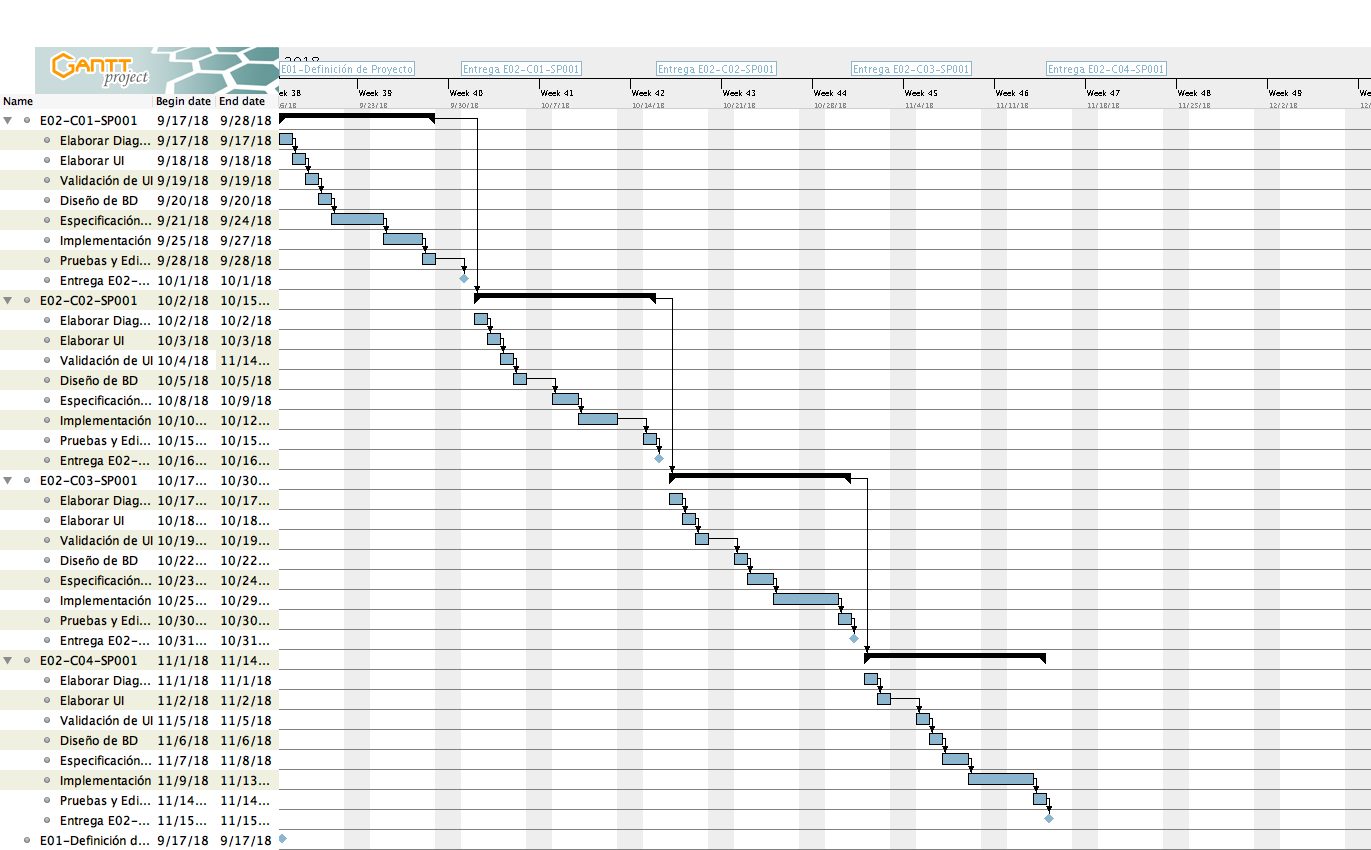
\includegraphics[angle=90,height=\textheight]{img/gantt}}
		\caption{Calendario de Actividades}
		\label{fig:cal}
	\end{center}
\end{figure}
